\documentclass[border=1mm]{standalone}
% \usepackage[margin=2.5cm]{geometry}

\usepackage{graphicx,tikz,tikz-layers,amsmath,ifthen,tabularray} 
\usetikzlibrary{decorations.markings,calc,positioning,arrows,shapes.geometric,arrows.meta,matrix}

\colorlet{myred}{red!80!black}
\colorlet{myblue}{blue!80!black}
\colorlet{mybluee}{myblue!80!black}
\colorlet{mygreen}{green!60!black}
\colorlet{myorange}{orange!70!red!60!black}
\colorlet{mydarkred}{red!20!black}
\colorlet{mydarkblue}{blue!40!black}
\colorlet{mydarkgreen}{green!20!black}




\begin{document}

% \resizebox{\textwidth}{!}{
\tikz[font=\footnotesize, scale=1, every node/.style={outer sep=0pt, inner sep=0pt, align=center, rounded corners=0mm}, w/.style={minimum width=#1}, h/.style={minimum height=#1}, s/.style={minimum size=#1}, eu/.style={shorten >=#1}, ed/.style={shorten <=#1}, line join=round]
{
\tikzset{>={Latex[length=1.5mm, width=1.25mm]}}

\node[] (image) {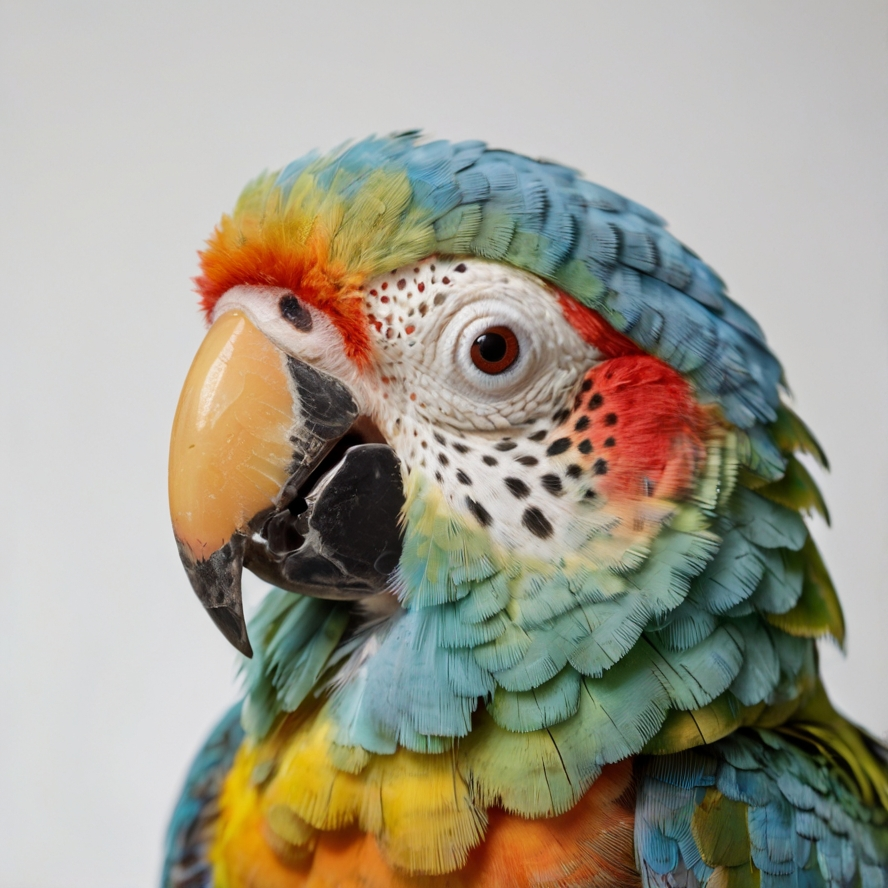
\includegraphics[width=2cm]{images/parrot3.jpg}};

\node[draw, w=.6cm, h=2.5cm, right=2.5cm of image, fill=myblue!20] (a1) {};
\node[draw, w=.6cm, h=2cm, right=.2cm of a1, fill=myblue!20] (a2) {};
\node[draw, w=.6cm, h=1.5cm, right=.2cm of a2, fill=myblue!20] (a3) {};
\node[draw, w=.6cm, h=1cm, right=.2cm of a3, fill=myblue!20] (a4) {};

\node[draw, w=.6cm, h=1cm, right=.2cm of a4, fill=myblue!20] (b1) {};
\node[draw, w=.6cm, h=1.5cm, right=.2cm of b1, fill=myblue!20] (b2) {};
\node[draw, w=.6cm, h=2cm, right=.2cm of b2, fill=myblue!20] (b3) {};
\node[draw, w=.6cm, h=2.5cm, right=.2cm of b3, fill=myblue!20] (b4) {};

\node[right=2.5cm of b4] (image2) {
\includegraphics[width=2cm]{images/noise.png}};

% ---
\node[draw, w=.2cm, h=1cm, fill=mygreen!20, anchor=north east] (a) at ($(a1.south west)+(0,-.5)$) {};
\node[draw, w=.2cm, h=1cm, fill=mygreen!20, left=1mm of a, label={[label distance=2mm, font=\footnotesize]below:Full-connected Layers}] (b) {};
\node[draw, w=.2cm, h=1cm, fill=mygreen!20, left=1mm of b] (c) {};

%---
\node[draw, s=.3cm, label={[label distance=2mm, font=\footnotesize]below:Time\\Representation}] (0) at (c-|image) {};
\node[draw, s=.3cm, right=0mm of 0] (1) {};
\node[draw, s=.3cm, right=0mm of 1] (2) {};
\node[draw, s=.3cm, left=0mm of 0] (-1) {};
\node[draw, s=.3cm, left=0mm of -1] (-2) {};

% Arrows and labels
\draw[->] ($(a1.west)+(-1.25,0)$)--node[pos=0,left=2mm] {$x_t$} (a1);
\draw[->] (b4.east)--node[pos=1,right=2mm] {$\epsilon_\theta(x_t,t)$} +(1,0);
\draw[->] ($(c.west)+(-.5,0)$)--node[pos=0,left=2mm] {$t$} (c);

\foreach \i in{a1,b1,a2,b2,a3,b3,a4,b4}
\draw[->] (a) -| (\i);



}

% }



\end{document}
